\documentclass{beamer}

\usetheme{Madrid} % Or choose another theme like Berlin, Warsaw, Singapore, etc.
\usecolortheme{default}

\usepackage{graphicx} % For including images
\usepackage{listings} % For code listings
\usepackage{textcomp} % For symbols like \textrightarrow

% Define code listing styles
\lstdefinestyle{customc}{
  language=C++,
  basicstyle=\scriptsize\ttfamily,
  keywordstyle=\color{blue},
  commentstyle=\color{green!70!black},
  stringstyle=\color{red},
  showstringspaces=false,
  breaklines=true,
  frame=tb,
  numbers=left,
  numberstyle=\tiny\color{gray},
}

\lstdefinestyle{custompy}{
  language=Python,
  basicstyle=\scriptsize\ttfamily,
  keywordstyle=\color{blue},
  commentstyle=\color{green!70!black},
  stringstyle=\color{red},
  showstringspaces=false,
  breaklines=true,
  frame=tb,
  numbers=left,
  numberstyle=\tiny\color{gray},
}

\lstdefinestyle{custommermaid}{
  language=Mermaid, % Assuming a simple text-based 'language' for mermaid
  basicstyle=\scriptsize\ttfamily,
  keywordstyle=\color{purple},
  breaklines=true,
  frame=tb,
}


\title[IntelliGaze]{IntelliGaze: A Wearable AI Camera System}
\subtitle{Real-time Environmental Description via AI and TTS}
\author[Seyam  , Eftekhar  , Mim  , Mahin  , Muntasir  ]{
    Touhidul Alam Seyam (230240003)\\ 
    Eftakar Uddin (230240004) \\ 
    Tasmim Akther Mim (230240025) \\ 
    Shafiul Azam Mahin (230240022) \\ 
    Muntasir Rahman (230240002)
}
\date{\today}
\institute{
    Microprocessor Lab \\ 
    Future Professor Radiathun Tasnia,\\ Junior Lecturer, \\ BGC Trust University Bangladesh
}

\begin{document}

% --- Title Frame ---
\begin{frame}
  \titlepage
\end{frame}

% --- Table of Contents ---
\begin{frame}{Outline}
  \tableofcontents
\end{frame}

% --- Introduction Section ---
\section{Introduction}

\begin{frame}{What is IntelliGaze?}
  \begin{columns}[T] % Align columns at the top
    \footnotesize
    \begin{column}{0.6\textwidth}
      \textbf{Core Idea:} An innovative project integrating an ESP32-CAM on goggles to capture and document moments using AI.
      \vspace{1em}
      \begin{itemize}
        \item Provides real-time auditory descriptions of the surroundings.
        \item Allows users to stream live video (implicitly).
        \item Generates scene descriptions via AI (Google Gemini).
        \item Aims for hands-free operation via a mobile app.
      \end{itemize}
       \vspace{1em}
       \textbf{Applications:}
       \begin{itemize}
        \item Assistive technology for the visually impaired.
        \item Contextual awareness tool.
        \item Personal memory archival (with descriptions).
      \end{itemize}
    \end{column}
    \begin{column}{0.4\textwidth}
      \centering
      \includegraphics[width=\linewidth]{"vision vault.jpeg"} \\ % Assuming image is in assets folder relative path needed or same folder
    \end{column}
  \end{columns}
\end{frame}

% --- Problem Statement Frame ---
\begin{frame}{Problem Statement}
  \frametitle{Challenges Addressed}
  \begin{itemize}
    \item Challenges faced by visually impaired individuals in navigating and understanding their environment.
    \item Need for real-time, hands-free contextual information.
    \item Desire for an accessible way to document and recall visual experiences.
    \item Existing assistive technologies may lack real-time AI-powered descriptive capabilities or seamless integration.
  \end{itemize}
\end{frame}

% --- Our Solution Frame ---
\begin{frame}{Our Solution: IntelliGaze}
  \frametitle{How IntelliGaze Helps}
  \begin{itemize}
    \item Provides immediate auditory feedback about the surroundings through AI analysis and TTS.
    \item Offers a wearable, hands-free experience via goggles and a mobile app.
    \item Leverages the power of Google Gemini for intelligent scene description.
    \item Creates a potential tool for enhanced independence and richer environmental interaction for the visually impaired.
    \item Serves as a novel personal memory archival system with generated context.
  \end{itemize}
\end{frame}

% --- Justification Frame ---
\begin{frame}{Justification}
  \frametitle{Why IntelliGaze is Needed}
  \begin{itemize}
    \item Addresses the limitations of existing assistive tools by providing real-time, AI-driven environmental descriptions.
    \item Leverages accessible hardware (ESP32-CAM) and powerful AI (Google Gemini) for a cost-effective yet capable solution.
    \item Offers a hands-free, wearable approach for seamless integration into daily life.
    \item Provides significant value for visually impaired users (enhanced navigation, safety, context) and broader applications (memory assistance, context awareness).
  \end{itemize}
\end{frame}

% --- Workflow Section ---
\section{System Workflow}

\begin{frame}{System Workflow Overview}
  \frametitle{ESP32 \textrightarrow Python Server \textrightarrow Mobile App \textrightarrow TTS}
    \begin{itemize}
        \item \textbf{ESP32-CAM:} Streams video continuously over local WiFi.
        \item \textbf{Python Backend Server:}
            \begin{itemize}
                \item Fetches stream (with reconnection).
                \item Runs WebSocket Server (WSS) for secure mobile app communication.
                \item Manages client state (active/inactive, description interval).
                \item \textbf{Automatic Mode:} Periodically checks for scene changes. If changed, sends frame to API, broadcasts description to active clients.
                \item Handles commands from app (`start`, `stop`, `set\_interval`, `describe\_now`).
            \end{itemize}
         \item \textbf{React Native Mobile App:}
            \begin{itemize}
                \item Connects securely to Python Server (WSS, with reconnection).
                \item UI: Start/Stop, Interval config, Describe Now, History, Status indicators.
                \item Sends commands to server.
                \item Receives descriptions/errors.
                \item Provides TTS output and Haptic feedback.
            \end{itemize}
    \end{itemize}
\end{frame}

% --- Architecture Section ---
\section{System Architecture}

\begin{frame}{System Architecture Diagram}
    \frametitle{Overall Component Interaction}
    \begin{figure}
        \centering
        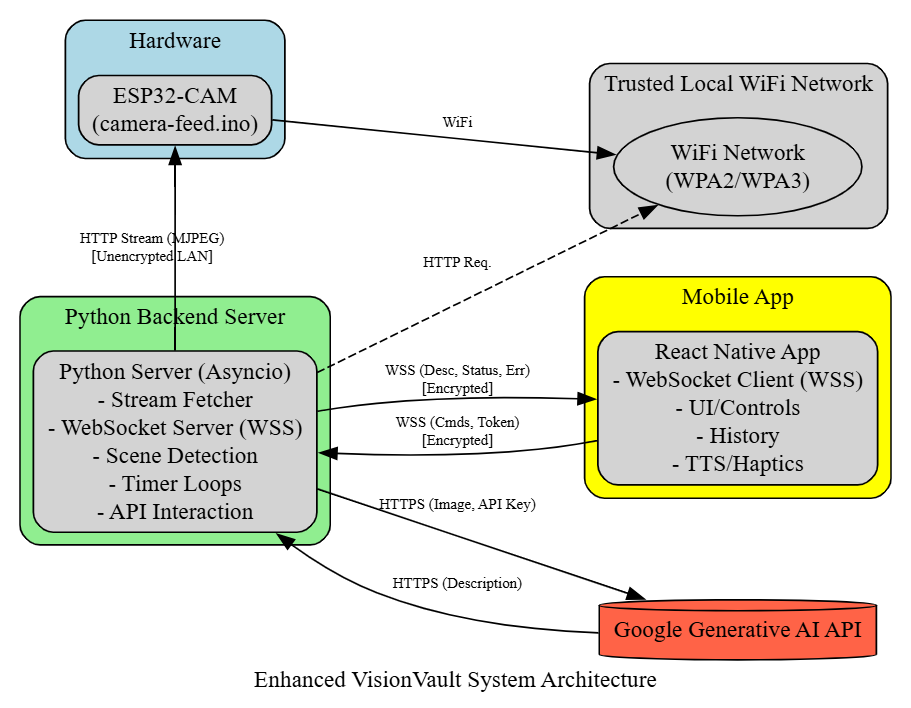
\includegraphics[width=0.75\textwidth]{Sys_Arch.png} % Use generated PNG
        \caption{High-level view of components and communication protocols.}
    \end{figure}
\end{frame}

\begin{frame}{Python Backend Server Internals}
    \frametitle{Modular Design}
     \begin{figure}
        \centering
        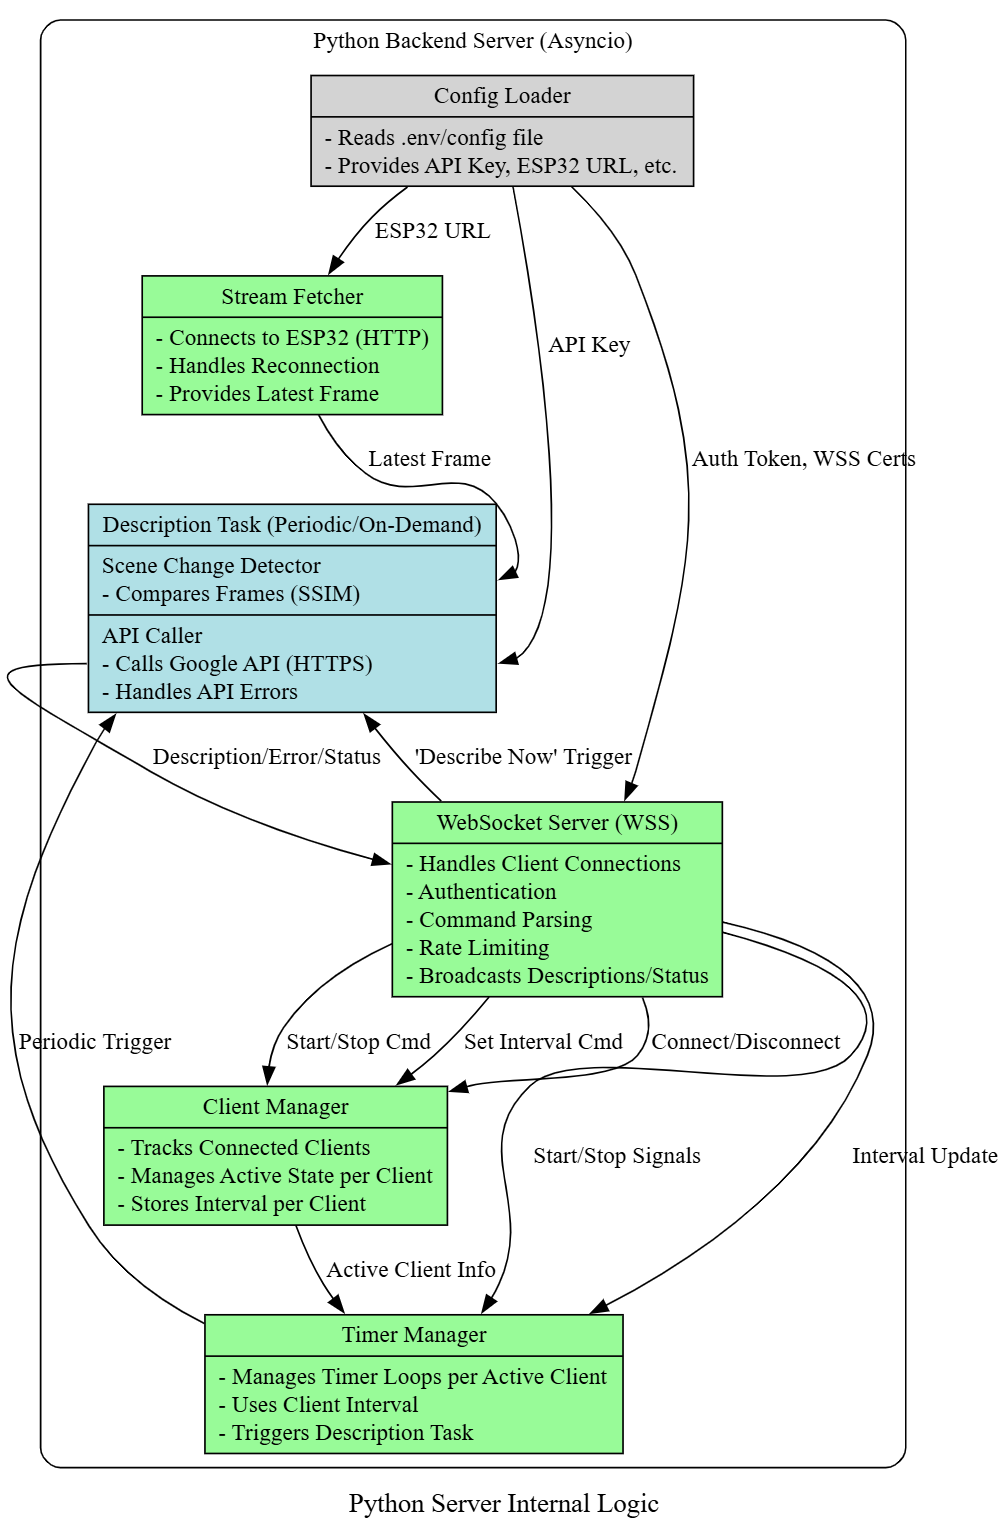
\includegraphics[height=0.75\textheight, width=0.8\textwidth, keepaspectratio]{Python_Server_Internal_Logic_Diagram.png} % Use generated PNG
        \caption{Key internal modules and data flow within the Python server.}
    \end{figure}
\end{frame}

\begin{frame}{Mobile App UI Flow}
    \frametitle{User Interaction States}
     \begin{figure}
        \centering
        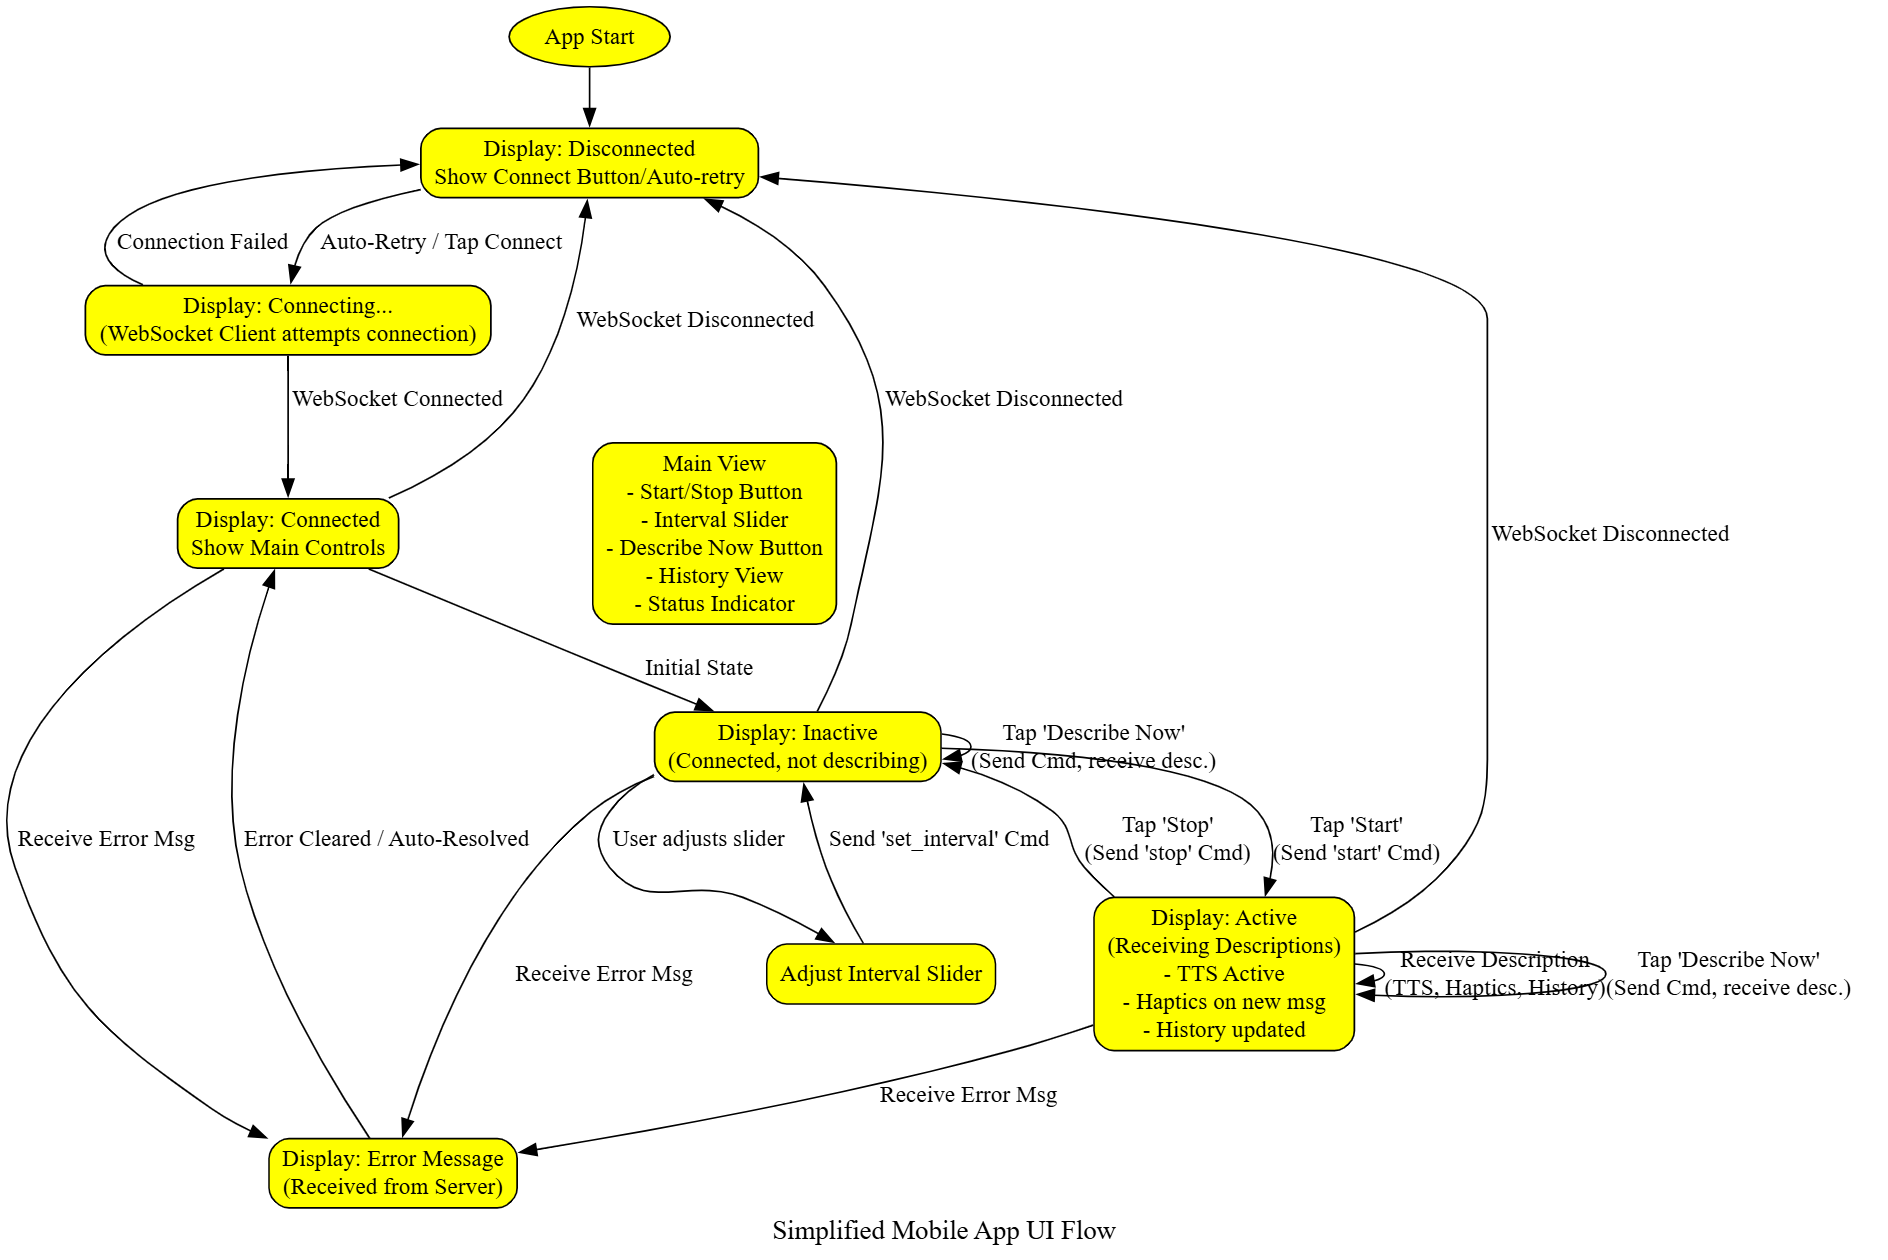
\includegraphics[height=0.75\textheight, width=\textwidth, keepaspectratio]{Mobile_App_UI_Flow_Diagram.png} % Use generated PNG
        \caption{Simplified state transitions within the React Native application.}
    \end{figure}
\end{frame}

% --- Core Logic Section ---
\section{Core Logic and Flows}

\begin{frame}{Algorithm: Scene Change Detection}
    \frametitle{Optimizing API Calls}
     \begin{figure}
        \centering
        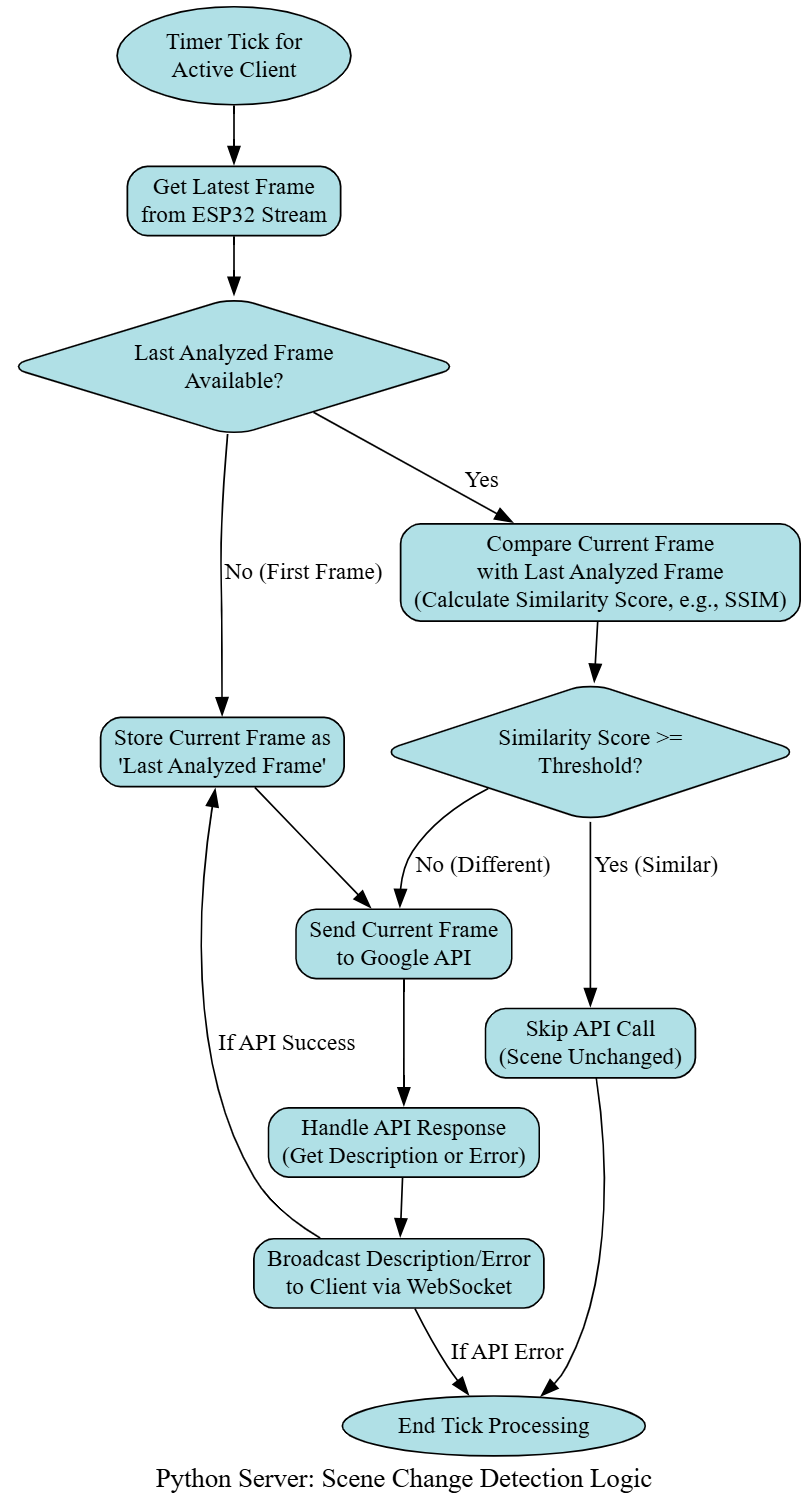
\includegraphics[height=0.8\textheight, width=0.6\textwidth, keepaspectratio]{Scene_Change_Detection_Logic_Flowchart.png} % Use generated PNG
        \caption{Flowchart for deciding whether to call the AI API based on frame similarity.}
    \end{figure}
\end{frame}

% --- Technology & Code Section ---


\begin{frame}{Security Flow: WSS Authentication}
  \frametitle{Connecting Securely}
   \begin{figure}
      \centering
      % Mermaid source can't be directly rendered, use the PNG
      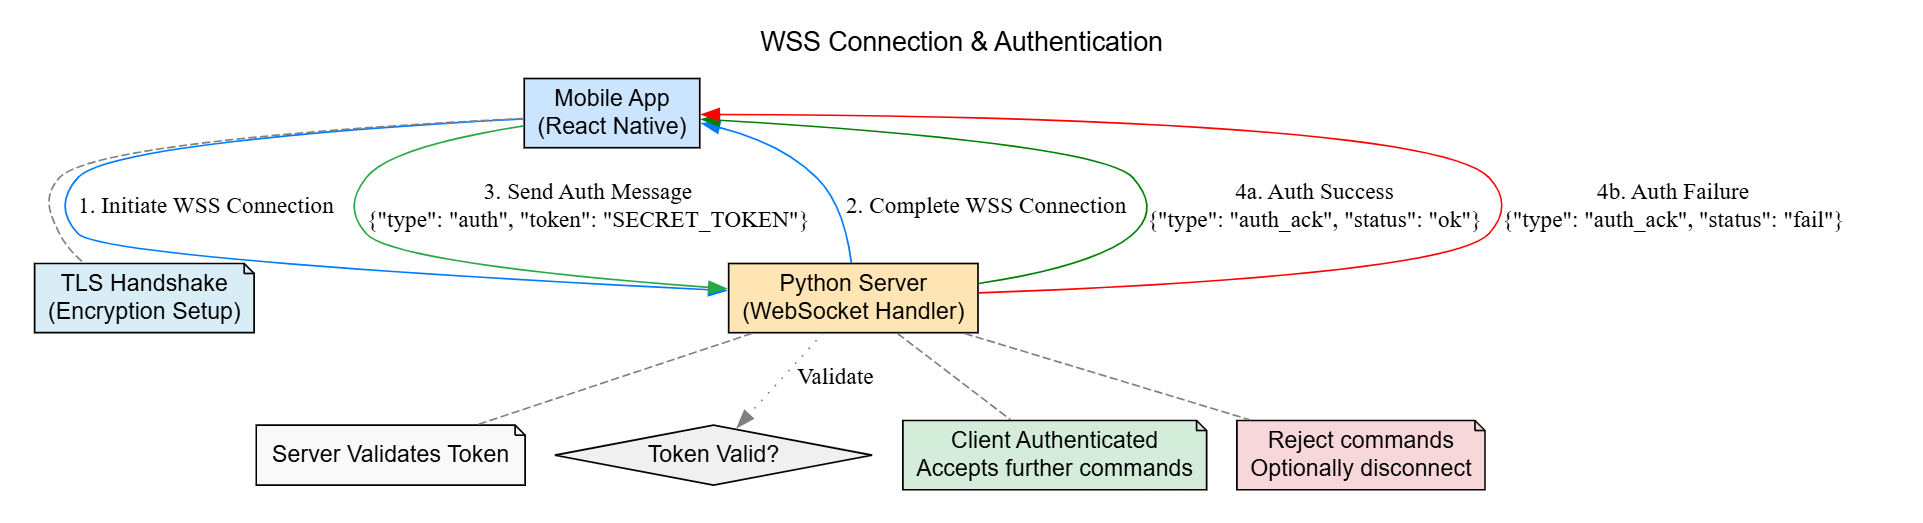
\includegraphics[width=0.9\textwidth, height=0.7\textheight, keepaspectratio]{Security_Flow_Diagram.png}
      \caption{Sequence for establishing a secure WebSocket connection with token authentication.}
  \end{figure}
\end{frame}


\section{Technology and Code}

\begin{frame}{Technology Stack}
    \frametitle{Key Technologies Used}
    \begin{itemize}
        \item \textbf{Hardware:} ESP32-CAM WiFi Module
        \item \textbf{Video Streaming:} MJPEG over HTTP
        \item \textbf{Backend:} Python 3 with `asyncio`, `websockets`, `aiohttp`/`requests`, `opencv-python`, `scikit-image` (for SSIM), `google-generativeai`, `python-dotenv`.
        \item \textbf{Frontend:} Expo React Native (TypeScript)
        \item \textbf{Communication:} Secure WebSockets (WSS)
        \item \textbf{AI:} Google Generative AI (Gemini API)
        \item \textbf{Output:} Text-to-Speech (TTS) Library (Expo TTS)
        \item \textbf{Feedback:} Haptics API (Expo Haptics)
    \end{itemize}
\end{frame}


% --- Security Section ---
\section{Security Aspects}

\begin{frame}{Security Considerations}
    \frametitle{Risks and Mitigations (Trusted LAN Focus)}
     \begin{itemize}
        \item \textbf{Network:} Assumes trusted WiFi (WPA2/WPA3). Public networks are risky.
        \item \textbf{ESP32 Stream (HTTP):} Unencrypted. Rely on WiFi security. HTTPS on ESP32 is challenging.
        \item \textbf{WebSocket (WSS):} \textit{Mitigation:} Use Secure WebSockets (`wss://`) with TLS certificates to encrypt app-server communication.
        \item \textbf{Authentication:} \textit{Mitigation:} Implement token-based authentication for WebSocket clients to prevent unauthorized access/commands.
        \item \textbf{API Key:} \textit{Mitigation:} Store securely (e.g., `.env` file, environment variables). Secure the host machine.
        \item \textbf{DoS:} \textit{Mitigation:} Implement rate limiting on WebSocket commands/connections on the server.
        \item \textbf{Input Validation:} \textit{Mitigation:} Sanitize all commands/data received from the mobile app on the server.
        \item \textbf{Resource Management:} Ensure server cleans up resources on client disconnect.
     \end{itemize}
\end{frame}




% --- Contributions Section ---
\section{Team Contributions}

\begin{frame}{Individual Contributions}
    \footnotesize
    \begin{itemize}
        \item \textbf{Touhidul Alam Seyam:} Will lead project design and integration. Will develop the core Python backend server including asynchronous stream handling, WebSocket communication (WSS), scene change detection, and Google Gemini API integration. Will implement core React Native application logic and features. Will design system architecture and workflow. Will create diagrams and presentation structure.

        \item \textbf{Eftakar Uddin:} Will configure and flash the ESP32-CAM firmware. Will conduct initial video stream testing and debugging. Will assist with Python server frame fetching setup.

        \item \textbf{Tasmim Akther Mim:} Will design and implement the user interface (UI) and user experience (UX) for the Expo React Native mobile application. Will integrate Text-to-Speech (TTS) and Haptics feedback components.

        \item \textbf{Shafiul Azam Mahin:} Will perform integration testing between the Python server, mobile app, and ESP32-CAM stream. Will research WebSocket libraries and will contribute to debugging network communication issues.

        \item \textbf{Muntasir Rahman:} Will contribute to project documentation. Will research Google Generative AI API capabilities and usage patterns relevant to the project. Will assist with overall system testing.
    \end{itemize}
\end{frame}

% --- Future Benefit Section ---
\section{Future Benefit}

\begin{frame}{Future Benefit}
    \frametitle{Potential Impact and Next Steps}
    \begin{itemize}
        \item \textbf{Enhanced Accessibility:} Potential for significant improvement in independence and quality of life for visually impaired individuals.
        \item \textbf{Broader Applications:} Can be adapted for augmented reality, professional training simulations, or automated documentation.
        \item \textbf{Technological Advancement:} Platform for integrating more sophisticated AI models (object recognition, activity detection), sensor fusion (adding audio, GPS), or cloud integration.
        \item \textbf{Personalization:} Future versions could learn user preferences or adapt descriptions based on context or location.
    \end{itemize}
\end{frame}

% --- Conclusion Section ---
\section{Conclusion}

\begin{frame}{Summary}
    \frametitle{IntelliGaze System Overview}
    \begin{itemize}
        \item A wearable system leveraging ESP32-CAM for continuous video input.
        \item Python backend processes the video, interacts with AI, and manages secure mobile app communication (WSS).
        \item Optimizes AI calls using scene change detection.
        \item React Native app provides user control (Start/Stop, Interval, On-Demand), displays history, and delivers auditory (TTS) / tactile (Haptic) feedback.
        \item Incorporates security measures for operation on trusted networks.
        \item Provides a robust framework for real-time, AI-driven environmental description.
    \end{itemize}
     \vspace{1em}
     \textbf{This design outlines the system; next steps involve implementation.}
\end{frame}


\end{document}
